%%%%%%%%%%%%%%%%%%%%%%%%%%%%%%%%%%%%%%%%%
% Jacobs Landscape Poster
% LaTeX Template
% Version 1.1 (14/06/14)
%
% Created by:
% Computational Physics and Biophysics Group, Jacobs University
% https://teamwork.jacobs-university.de:8443/confluence/display/CoPandBiG/LaTeX+Poster
% 
% Further modified by:
% Nathaniel Johnston (nathaniel@njohnston.ca)
%
% This template has been downloaded from:
% http://www.LaTeXTemplates.com
%
% License:
% CC BY-NC-SA 3.0 (http://creativecommons.org/licenses/by-nc-sa/3.0/)
%
%%%%%%%%%%%%%%%%%%%%%%%%%%%%%%%%%%%%%%%%%

%----------------------------------------------------------------------------------------
%	PACKAGES AND OTHER DOCUMENT CONFIGURATIONS
%----------------------------------------------------------------------------------------

\documentclass[final]{beamer}

%\usepackage[scale=1.]{beamerposter} % Use the beamerposter package for laying out the poster
\usepackage[scale=1]{beamerposter}

\usetheme{confposter} % Use the confposter theme supplied with this template

\setbeamercolor{block title}{fg=dblue,bg=white} % Colors of the block titles
\setbeamercolor{block body}{fg=black,bg=white} % Colors of the body of blocks
\setbeamercolor{block alerted title}{fg=white,bg=dblue!70} % Colors of the highlighted block titles
\setbeamercolor{block alerted body}{fg=black,bg=dblue!10} % Colors of the body of highlighted blocks
% Many more colors are available for use in beamerthemeconfposter.sty

%-----------------------------------------------------------
% Define the column widths and overall poster size
% To set effective sepwid, onecolwid and twocolwid values, first choose how many columns you want and how much separation you want between columns
% In this template, the separation width chosen is 0.024 of the paper width and a 4-column layout
% onecolwid should therefore be (1-(# of columns+1)*sepwid)/# of columns e.g. (1-(4+1)*0.024)/4 = 0.22
% Set twocolwid to be (2*onecolwid)+sepwid = 0.464
% Set threecolwid to be (3*onecolwid)+2*sepwid = 0.708

\newlength{\sepwid}
\newlength{\onecolwid}
\newlength{\twocolwid}
\newlength{\threecolwid}
\setlength{\paperwidth}{48in} % A0 width: 46.8in
\setlength{\paperheight}{36in} % A0 height: 33.1in
\setlength{\sepwid}{0.024\paperwidth} % Separation width (white space) between columns
\setlength{\onecolwid}{0.22\paperwidth} % Width of one column
\setlength{\twocolwid}{0.464\paperwidth} % Width of two columns
\setlength{\threecolwid}{0.708\paperwidth} % Width of three columns
\setlength{\topmargin}{-0.5in} % Reduce the top margin size
%-----------------------------------------------------------

\usepackage{graphicx}  % Required for including images

\usepackage{booktabs} % Top and bottom rules for tables

\usepackage{amsmath}
\usepackage{algorithm}
\usepackage[noend]{algpseudocode}
\usepackage{tikz}
\usepackage{verbatim}
\usepackage{caption}
\usepackage{textcomp}


%----------------------------------------------------------------------------------------
%	TITLE SECTION 
%----------------------------------------------------------------------------------------

\title{Coordinated Multi-Agent Control \\ Utilizing Deep Reinforcement Learning} % Poster title

\author{Alex Gao, Kevin Frans} % Author(s)

\institute{Henry M. Gunn High School} % Institution(s)

%----------------------------------------------------------------------------------------
\begin{document}

\addtobeamertemplate{block end}{}{\vspace*{2ex}} % White space under blocks
\addtobeamertemplate{block alerted end}{}{\vspace*{2ex}} % White space under highlighted (alert) blocks

\setlength{\belowcaptionskip}{2ex} % White space under figures
\setlength\belowdisplayshortskip{2ex} % White space under equations

\begin{frame}[t] % The whole poster is enclosed in one beamer frame

\begin{columns}[t] % The whole poster consists of three major columns, the second of which is split into two columns twice - the [t] option aligns each column's content to the top

\begin{column}{\sepwid}\end{column} % Empty spacer column

\begin{column}{\onecolwid} % The first column

\begin{block}{Introduction}

In today's world, nearly everything is automated. But behind this veil of automation, a programmer has to explicitly tell the computer how to act in each situation. As more complex problems are reached, this manual method becomes impractical, as it requires excessive amounts of work.
\\[12pt]
With autonomous learning, we allow the computer to figure out a strategy on its own. This strategy is referred to as a \textbf{policy}, and the computer program following it is an \textbf{agent}.
\\[12pt]
In a standard setup, many simulations are run on an unknown task, starting from a random policy. How the simulation data can be used to improve the policy is an active area of research, especially with the rise of modern computing power.
\end{block}

\begin{alertblock}{Objectives}

In this experiment, our goal is to identify new learning methods in order to:

    \begin{itemize}
    \item Improve performance on the task. Each task defines success in a different manner, and an optimal strategy may involve cooperation between multiple agents.

    \item Speed up training time. An algorithm that requires less simulations can learn at a faster rate. Additionally, algorithms that require less compute power can be executed faster in terms of wall-clock time.
    
    \end{itemize}

\end{alertblock}

\begin{block}{Reinforcement Learning}

When a human child learns to walk, it isn't told how. Instead, the child keeps trying things until it figures out how each of its muscles should move. Reinforcement learning, a subset of machine learning, follows the same methodology. Through continuous trial and error, a policy can gradually be improved upon.
\\[12pt]
We represent our policy as a \textbf{deep neural network}, mapping from an observation vector (positions and angles of joints) to an agent's actions (joint torque). The policy is stochastic: actions are represented as normal distributions, parametrized by a mean and a standard deviation. This network can be thought of as an agent's "brain".
\\[12pt]
Each task gives out a reward value based on how well the agent is performing. This reward is different in each task, ranging from 'how far forward the agent has traveled' to 'how close is the agent to a desired point'.
\\[12pt]
By repeatedly running simulations of a task, we can record which actions, on average, resulted in a higher reward.
\\[12pt]
Utilizing this information, we backpropagate through the neural network, increasing the likelihood of actions that have proven to be beneficial.
\\[12pt]
This paradigm is known as the \textbf{policy gradient}, and is the basis for how our learning agent is trained.


\end{block}

\end{column} % End of the first column

\begin{column}{\sepwid}\end{column} % Empty spacer column

\begin{column}{\twocolwid} % Begin a column which is two columns wide (column 2)




%----------------------------------------------------------------------------------------

\begin{columns}[t,totalwidth=\twocolwid] % Split up the two columns wide column again

\begin{column}{\onecolwid} % The first column within column 2 (column 2.1)

%----------------------------------------------------------------------------------------
%	MATHEMATICAL SECTION
%----------------------------------------------------------------------------------------

\vspace{-1.3cm}

\begin{block}{Hypothesis}

Traditional methods use one big policy to account for all the agents actions. 
However, this setup has trouble scaling into more complex tasks. \textbf{Instead, we split this large network into many smaller, distinct networks --- one for each agent.} We view each of a robot's joints as separate agents, allowing independent decisions to be made. In practice, this means training distinct neural networks for each joint. Our method is \textbf{decentralized}, and each network can be trained and executed independently of the others.
	
\begin{figure}
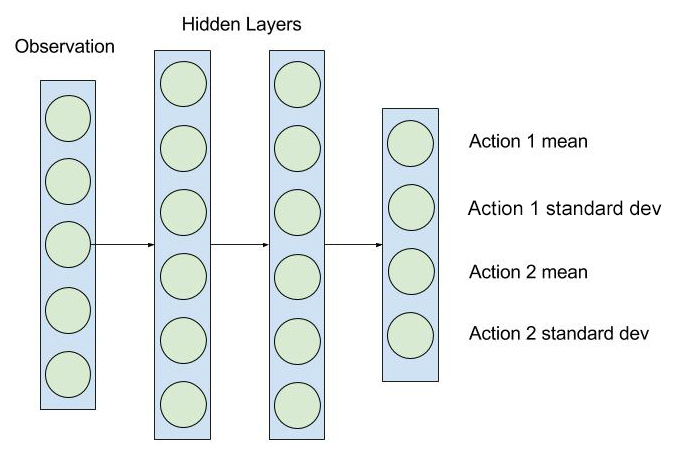
\includegraphics[width=0.4\linewidth]{syn-regnet.jpg}
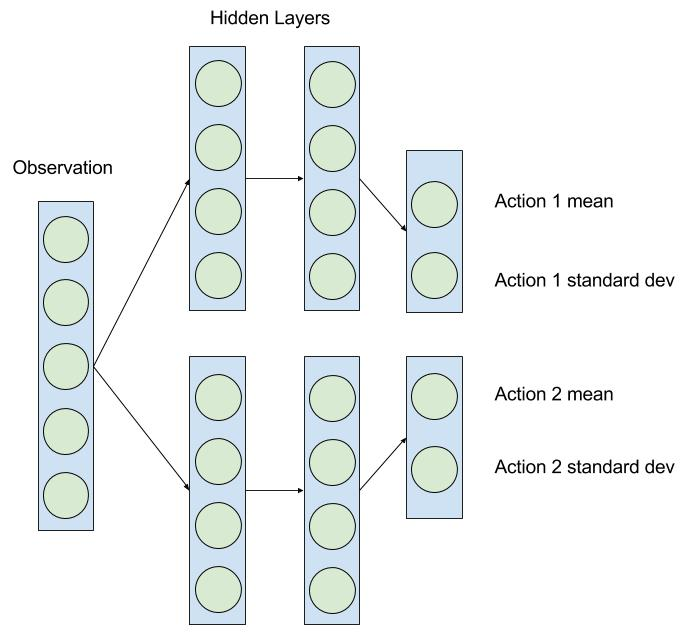
\includegraphics[width=0.4\linewidth]{syn-splitnet.jpg}
\caption{Left: traditional network. Right: decentralized network.}
\end{figure}

\end{block}


\begin{block}{Tasks}

\begin{figure}
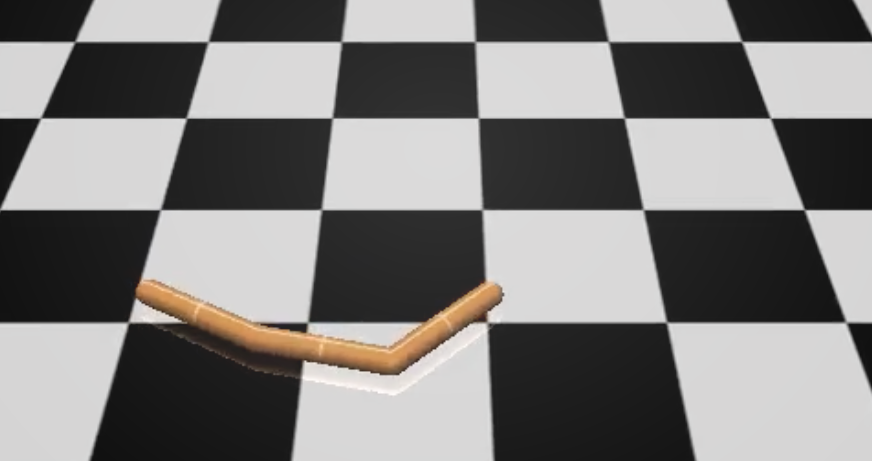
\includegraphics[width=0.5\linewidth]{swimmerenv.png}
\caption{Swimmer}
\end{figure}

\begin{figure}
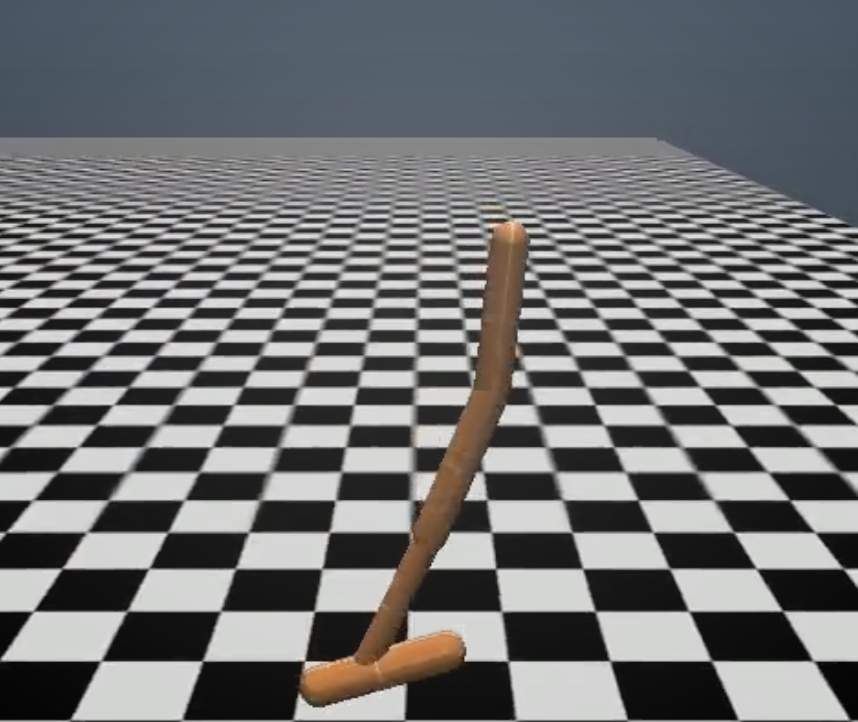
\includegraphics[width=0.5\linewidth]{hopperenv.png}
\caption{Hopper}
\end{figure}

\begin{figure}
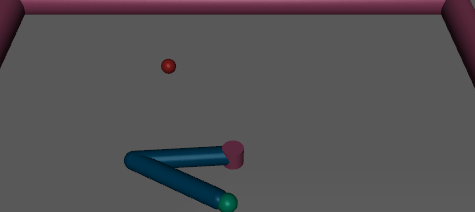
\includegraphics[width=0.5\linewidth]{reacherenv.png}
\caption{Reacher}
\end{figure}

\begin{figure}
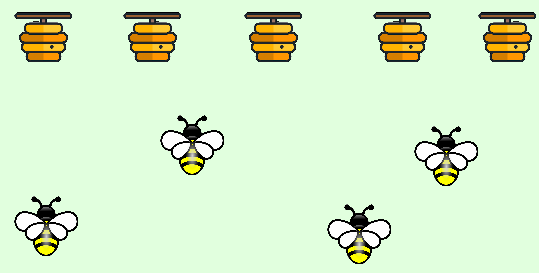
\includegraphics[width=0.5\linewidth]{deliveryenv.png}
\caption{Delivery}
\end{figure}

\end{block}


\end{column} % End of column 2.1



\begin{column}{\onecolwid} % The second column within column 2 (column 2.2)

\vspace{-1.3cm}

\begin{block}{Rationale}

Large neural networks, especially those with multiple objectives, often struggle to encode observations correctly. For example, a robot will move its leg joint differently, depending on the position of its foot. However, this information is not useful in controlling its right arm. When using a single network, the network is forced to encode all information, which can lead to confusion.
\\[12pt]
By utilizing multiple networks, we allow \textbf{each network to specialize}, and only encode the information useful to its specific role in the task.
\\[12pt]
Additionally, the decentralization of our policy enables scaling up of training, through \textbf{parallelization}. In a centralized setup, the entire network would have to be updated before the next update could start. With the policy split into separate networks, each can be trained on different computers, in parallel -- allowing for faster training when scaling up.

\end{block}


\begin{block}{Results}

    \begin{figure}
    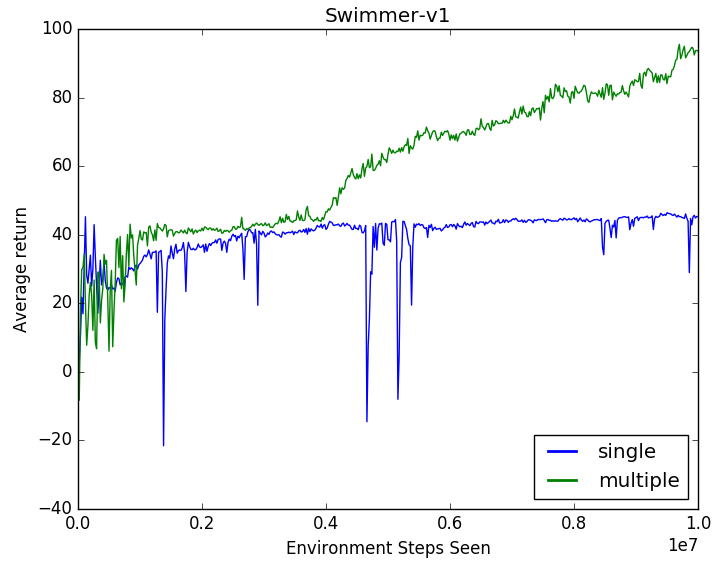
\includegraphics[width=0.5\linewidth]{swimmer.png}
    \end{figure}

    \begin{figure}
    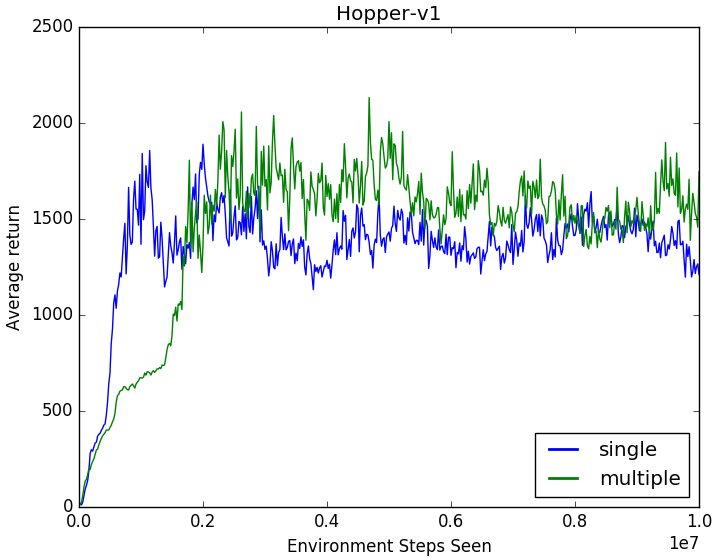
\includegraphics[width=0.5\linewidth]{hopper.png}
    \end{figure}

    \begin{figure}
    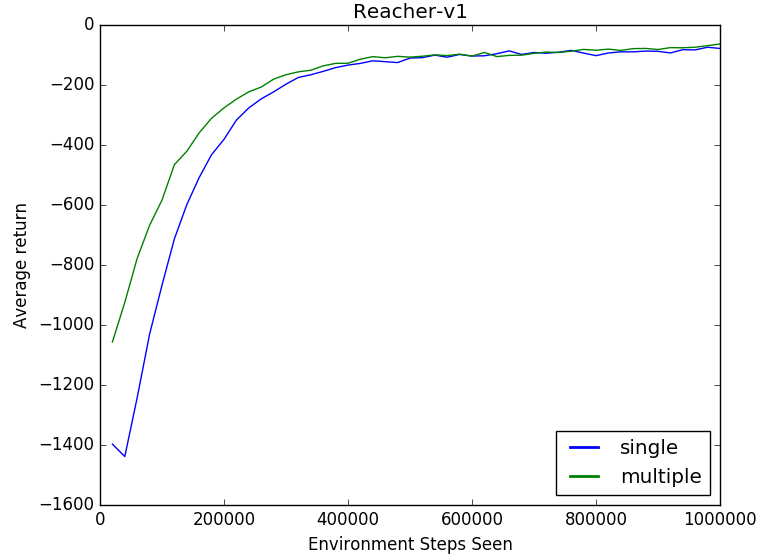
\includegraphics[width=0.5\linewidth]{reacher.png}
    \end{figure}

    \begin{figure}
    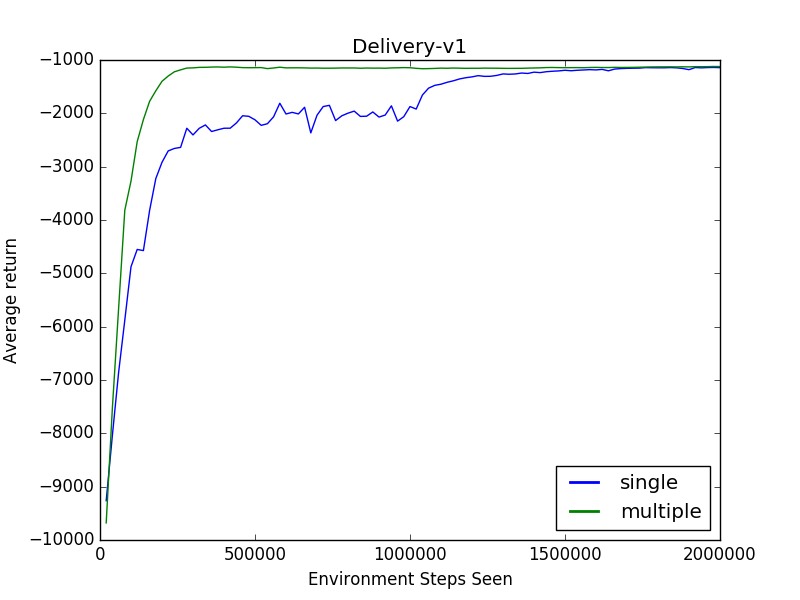
\includegraphics[width=0.5\linewidth]{delivery.png}
    \end{figure}


\end{block}


%----------------------------------------------------------------------------------------

\end{column} % End of column 2.2

\end{columns} % End of the split of column 2

\end{column} % End of the second column

\begin{column}{\sepwid}\end{column} % Empty spacer column

\begin{column}{\onecolwid} % The third column

\begin{block}{Algorithm}

    \begin{algorithm}[H]
        \caption{Decentralized Policy Gradient}\label{euclid}
        \small
        \begin{algorithmic}[1]
            \State initialize $\pi$ for every agent
            \For{iteration = 0,1,2,... \text{until convergence}}
                \For{episode = 0,1,2, ... 10000}
                    \State Reset environment
                    \For{timestep = 0,1,2,... \text{until episode end}}
                        \State Receive observation
                        \State Every agent takes action according to policy $\pi$
                        \State Record tuple (observation, action, reward)
                        \EndFor
                \State Estimate value function Q(s,a) using recorded tuples
                \State Compute gradient to increase expected value
                \State Update policies in gradient direction
                \EndFor
            \EndFor

        \end{algorithmic}
    \end{algorithm}

\end{block}

\begin{block}{Conclusion}

We tested our algorithm's performance on a variety of standard control tasks, and showed an \textbf{increase of up to two times the performance of the single-network method}. Our method also learned an optimal solution in less simulations. Repeated trials on each task validated our results. 
\\[12pt]
While the total computational power of a decentralized method may be higher, the neural networks can be trained in parallel across multiple computers, effectively reducing the computational time. This is more beneficial for practical use, since the smaller neural networks can be distributed among each agent without intercommunication.
\\[12pt]
Our method's improvements on the industry standard, in terms of performance and training time, allow for deep reinforcement learning to be applied in many practical scenarios. Real-world problems such as assembly line robotics have traditionally been explicitly coded; however, as autonomous learning becomes more efficient, artificial intelligence may take over these jobs.


\end{block}

%----------------------------------------------------------------------------------------
%	ADDITIONAL INFORMATION
%----------------------------------------------------------------------------------------

\begin{block}{Future Work}
Our work provides a reliable basis for practical cooperative learning in a multitude of environments, and paves the way for future research in the emergent field of multi-agent control.
\\[12pt]
Our robust algorithm has countless practical applications requiring cooperative learning that can be explored in future work, including:

\begin{itemize}
\item Drone package delivery network management and collision avoidance
\item Robotic bee pollination to proxy bee extinction
\item Planetary exploration with teams of rovers
\item Prosthetics for disabled persons
\end{itemize}

\end{block}



%\begin{block}{References}

%\nocite{*} % Insert publications even if they are not cited in the poster
%\small{\bibliographystyle{unsrt}
%\bibliography{sample}\vspace{0.75in}}

%\end{block}




%----------------------------------------------------------------------------------------

\end{column} % End of the third column

\end{columns} % End of all the columns in the poster

\end{frame} % End of the enclosing frame

\end{document}
